\documentclass{beamer}

\pdfmapfile{+sansmathaccent.map}


\mode<presentation>
{
	\usetheme{Warsaw} % or try Darmstadt, Madrid, Warsaw, Rochester, CambridgeUS, ...
	\usecolortheme{seahorse} % or try seahorse, beaver, crane, wolverine, ...
	\usefonttheme{serif}  % or try serif, structurebold, ...
	\setbeamertemplate{navigation symbols}{}
	\setbeamertemplate{caption}[numbered]
} 


%%%%%%%%%%%%%%%%%%%%%%%%%%%%
% itemize settings

\definecolor{mypaleblue}{RGB}{240, 240, 255}
\definecolor{mylightblue}{RGB}{120, 150, 255}
\definecolor{myblue}{RGB}{90, 90, 255}
\definecolor{mygblue}{RGB}{70, 110, 240}
\definecolor{mydarkblue}{RGB}{0, 0, 180}
\definecolor{myblackblue}{RGB}{40, 40, 120}

\definecolor{mygreen}{RGB}{0, 200, 0}
\definecolor{mydarkgreen}{RGB}{0, 120, 0}
\definecolor{mygreen2}{RGB}{245, 255, 230}

\definecolor{mygray}{gray}{0.8}
\definecolor{mygray2}{RGB}{130, 130, 130}
\definecolor{mydarkgray}{RGB}{80, 80, 160}
\definecolor{mylightgray}{RGB}{160, 160, 160}

\definecolor{mydarkred}{RGB}{160, 30, 30}
\definecolor{mylightred}{RGB}{255, 150, 150}
\definecolor{myred}{RGB}{200, 110, 110}
\definecolor{myblackred}{RGB}{120, 40, 40}

\definecolor{mypink}{RGB}{255, 30, 80}
\definecolor{myhotpink}{RGB}{255, 80, 200}
\definecolor{mywarmpink}{RGB}{255, 60, 160}
\definecolor{mylightpink}{RGB}{255, 80, 200}
\definecolor{mydarkpink}{RGB}{155, 25, 60}

\definecolor{mydarkcolor}{RGB}{60, 25, 155}
\definecolor{mylightcolor}{RGB}{130, 180, 250}

\setbeamertemplate{itemize items}[default]

\setbeamertemplate{itemize item}{\color{myblackblue}$\blacksquare$}
\setbeamertemplate{itemize subitem}{\color{mydarkblue}$\blacktriangleright$}
\setbeamertemplate{itemize subsubitem}{\color{mygray}$\blacksquare$}

\setbeamercolor{palette quaternary}{fg=white,bg=mygblue} %mydarkgray
\setbeamercolor{titlelike}{parent=palette quaternary}

\setbeamercolor{palette quaternary2}{fg=white,bg=mygblue}%black myblue
\setbeamercolor{frametitle}{parent=palette quaternary2}

\setbeamerfont{frametitle}{size=\Large,series=\scshape}
\setbeamerfont{framesubtitle}{size=\normalsize,series=\upshape}


%%%%%%%%%%%%%%%%%%%%%%%%%%%%
% block settings

%\setbeamercolor{block title}{bg=red!50,fg=black}
%\setbeamercolor{block title}{bg=mylightblue,fg=black}
\setbeamercolor{block title}{bg=myblackblue,fg=white}

\setbeamercolor*{block title example}{bg=mygreen!40!white,fg=black}

\setbeamercolor*{block body example}{fg= black,
	bg= mygreen2}


%%%%%%%%%%%%%%%%%%%%%%%%%%%%
% URL settings
\hypersetup{
	colorlinks=false,
	linkcolor=blue,
	filecolor=blue,      
	urlcolor=blue,
}

%%%%%%%%%%%%%%%%%%%%%%%%%%

\renewcommand{\familydefault}{\rmdefault}

\usepackage{amsmath}
\usepackage{mathtools}

\usepackage{subcaption}

\usepackage{qrcode}

\newcommand{\bo}[1] {\mathbf{#1}}
\newcommand{\R}{\mathbb{R}} 
\newcommand{\T}{^\top}     



\newcommand{\mydate}{Spring 2025}

\newcommand{\mygit}{\textcolor{blue}{\href{https://github.com/SergeiSa/Computational-Intelligence-2025}{github.com/SergeiSa/Computational-Intelligence-2025}}}

\newcommand{\myqr}{ \textcolor{black}{\qrcode[height=1.5in]{https://github.com/SergeiSa/Computational-Intelligence-2025}}
}

\newcommand{\myqrframe}{
	\begin{frame}
		\centerline{Lecture slides are available via Github, links are on Moodle:}
		\bigskip
		\centerline{\mygit}
		\bigskip
		\myqr
	\end{frame}
}


\newcommand{\bref}[2] {\textcolor{blue}{\href{#1}{#2}}}



%%%%%%%%%%%%%%%%%%%%%%%%%%%%
% code settings

\usepackage{listings}
\usepackage{color}
% \definecolor{mygreen}{rgb}{0,0.6,0}
% \definecolor{mygray}{rgb}{0.5,0.5,0.5}
\definecolor{mymauve}{rgb}{0.58,0,0.82}
\lstset{ 
	backgroundcolor=\color{white},   % choose the background color; you must add \usepackage{color} or \usepackage{xcolor}; should come as last argument
	basicstyle=\footnotesize,        % the size of the fonts that are used for the code
	breakatwhitespace=false,         % sets if automatic breaks should only happen at whitespace
	breaklines=true,                 % sets automatic line breaking
	captionpos=b,                    % sets the caption-position to bottom
	commentstyle=\color{mygreen},    % comment style
	deletekeywords={...},            % if you want to delete keywords from the given language
	escapeinside={\%*}{*)},          % if you want to add LaTeX within your code
	extendedchars=true,              % lets you use non-ASCII characters; for 8-bits encodings only, does not work with UTF-8
	firstnumber=0000,                % start line enumeration with line 0000
	frame=single,	                   % adds a frame around the code
	keepspaces=true,                 % keeps spaces in text, useful for keeping indentation of code (possibly needs columns=flexible)
	keywordstyle=\color{blue},       % keyword style
	language=Octave,                 % the language of the code
	morekeywords={*,...},            % if you want to add more keywords to the set
	numbers=left,                    % where to put the line-numbers; possible values are (none, left, right)
	numbersep=5pt,                   % how far the line-numbers are from the code
	numberstyle=\tiny\color{mygray}, % the style that is used for the line-numbers
	rulecolor=\color{black},         % if not set, the frame-color may be changed on line-breaks within not-black text (e.g. comments (green here))
	showspaces=false,                % show spaces everywhere adding particular underscores; it overrides 'showstringspaces'
	showstringspaces=false,          % underline spaces within strings only
	showtabs=false,                  % show tabs within strings adding particular underscores
	stepnumber=2,                    % the step between two line-numbers. If it's 1, each line will be numbered
	stringstyle=\color{mymauve},     % string literal style
	tabsize=2,	                   % sets default tabsize to 2 spaces
	title=\lstname                   % show the filename of files included with \lstinputlisting; also try caption instead of title
}

%%%%%%%%%%%%%%%%%%%%%%%%%%%%
% tikz settings

\usepackage{tikz}
\tikzset{every picture/.style={line width=0.75pt}}

%%%%%%%%%%%%%%%%%%%%%%%%%%%%




\title{Linear Programming}
\subtitle{Computational Intelligence, Lecture 6}
\author{by Sergei Savin}
\centering
\date{\mydate}

\begin{document}
\maketitle


\begin{frame}{Content}

\begin{itemize}
\item Linear Programming
\item Convex piece-wise linear functions
\item Chebyshev center of a polyhedron
\item Linear-Fractional Programming
\item Homework
\end{itemize}

\end{frame}



\begin{frame}{Linear Programming}
\begin{flushleft}

A linear program (LP) is an optimization problem of the form:

\begin{equation} \label{LP}
	\begin{aligned}
		& \underset{\bo{x}}{\text{minimize}}
		& & \bo{f}^\top \bo{x} , \\
		& \text{subject to}
		& & \begin{cases} 
			\bo{A}\bo{x} \leq \bo{b}, \\
			\bo{C}\bo{x} = \bo{d}.
		\end{cases}
		%
	\end{aligned}
\end{equation}

It is one of the older and widely used classes of convex optimization problems. 

\bigskip

Note that the solution of such problem will always lie on the boundary of its domain.
 
\end{flushleft}
\end{frame}



\begin{frame}{LP - simpler formulations, 1}
	\begin{flushleft}
		
		Inequality $\bo{A}\bo{x} \leq \bo{b}$ can be re-written as a combination of two constraints: $\bo{A}\bo{x} - \bo{b} = -\bo{z}$ and $\bo{z} \geq 0$. Thus, we can re-write the LP as:
		
		
		\begin{equation}
			\begin{aligned}
				& \underset{\bo{x}, \bo{z}}{\text{minimize}}
				& & \bo{f}^\top \bo{x} , \\
				& \text{subject to}
				& & \begin{cases} 
					\bo{A}\bo{x} - \bo{z} = \bo{b}, \\
					\bo{C}\bo{x} = \bo{d}, \\
					\bo{z} \geq 0
				\end{cases}
				%
			\end{aligned}
		\end{equation}
		
		Domain of the variable $\bo{x}$ is $\mathbb{X} = \{ \bo{x}:  \R^n \}$ and the domain of the variable $\bo{z}$ is $\mathbb{Z} = \{ \bo{z}:  \bo{z} \geq 0 \}$.
		
		\bigskip 
		
		Domain of the entire proble can be described as direct sum $\mathbb{X}  \oplus \mathbb{Z}$ intersected by the hyperplane 
		$
		\begin{bmatrix}
			\bo{A} & - \bo{I} \\
			\bo{C} & \bo{0}
		\end{bmatrix}
		\begin{bmatrix}
			\bo{x} \\
			\bo{z} 
		\end{bmatrix}
		=
		\begin{bmatrix}
			\bo{b} \\
			\bo{d}
		\end{bmatrix}
		$.
		
	\end{flushleft}
\end{frame}



\begin{frame}{LP - simpler formulations, 2}
	\begin{flushleft}
		
		Equality $\bo{C}\bo{x} = \bo{d}$ can be solved as $\bo{x} = \bo{C}^+\bo{d} + \bo{N}\bo{y}$. Thus, we can re-write the inequality $\bo{A}\bo{x} \leq \bo{b}$ as:
		
		\begin{align}
			\bo{A}(\bo{C}^+\bo{d} + \bo{N}\bo{y})  \leq \bo{b} 
			\\
			\bo{A}\bo{N}\bo{y}  \leq \bo{b} - \bo{A}\bo{C}^+\bo{d} 
			\\
			\bo{A}\bo{N}\bo{y}  \leq \bo{b}_0
		\end{align}
		%
		where $\bo{b}_0 = \bo{b} - \bo{A}\bo{C}^+\bo{d} $. Thus we get LP in the following form:
		
		\begin{equation}
			\begin{aligned}
				& \underset{\bo{y}}{\text{minimize}}
				& & \bo{f}^\top \bo{N}\T \bo{y} , \\
				& \text{subject to}
				& & \bo{A}\bo{N}\bo{y}  \leq \bo{b}_0
				%
			\end{aligned}
		\end{equation}
		
		Domain of this problem is a polytope $\bo{A}\bo{N}\bo{y}  \leq \bo{b}_0$.
		
	\end{flushleft}
\end{frame}




\begin{frame}{LP geometry}
	\begin{flushleft}
		
		% TODO: \usepackage{graphicx} required
		\begin{figure}
			\centering
			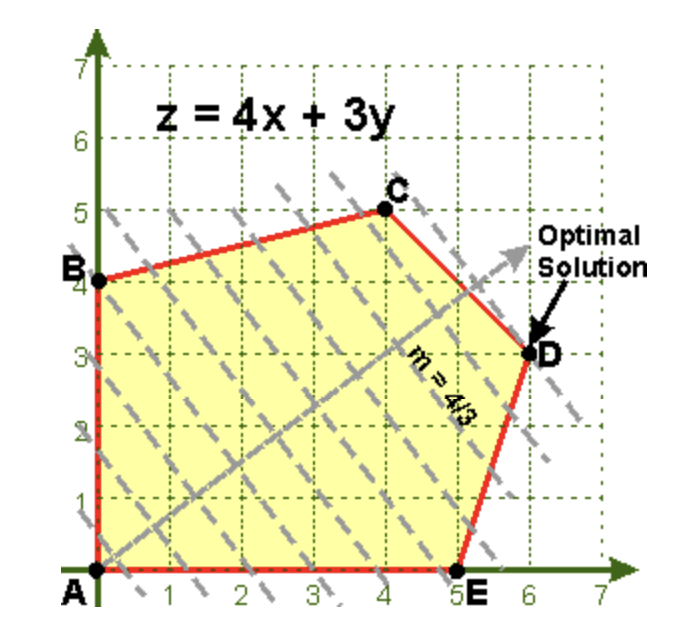
\includegraphics[width=0.70\linewidth]{LP_domain}
			\caption{Geometry of an LP problem - example.  \bref{https://people.richland.edu/james/lecture/m116/systems/linear.html}{Credit} }
			\label{fig:lpdomain}
		\end{figure}
		
		
	\end{flushleft}
\end{frame}






\begin{frame}{Linear Programming}
\framesubtitle{LP with no solution - examples}
\begin{flushleft}

Here are some examples of LP which have no solutions:

\begin{equation}
\begin{aligned}
& \underset{\mathbf{x}}{\text{minimize}}
& & \begin{bmatrix} 1 & 1 \end{bmatrix} 
\begin{bmatrix} x_1 \\ x_2 \end{bmatrix}
\end{aligned}
\end{equation}

This one is has no boundaries at all, hence no solution. Next one has boundaries, but they do not restrict motion along the descent direction for the cost function.

\begin{equation}
\begin{aligned}
& \underset{\mathbf{x}}{\text{minimize}}
& & \begin{bmatrix} 1 & 1 \end{bmatrix} 
\begin{bmatrix} x_1 \\ x_2 \end{bmatrix} , \\
& \text{subject to}
& & \begin{bmatrix} 1 & 0 \end{bmatrix}
\begin{bmatrix} x_1 \\ x_2 \end{bmatrix} \leq
1
%
\end{aligned}
\end{equation}

 
\end{flushleft}
\end{frame}



\begin{frame}{Convex piece-wise linear functions}
\framesubtitle{Problem statement}
\begin{flushleft}

Convex piece-wise linear functions have the form:

\begin{equation}
    f(\mathbf{x}) = \text{max}(\mathbf{a}_i^\top \mathbf{x} + b_i)
\end{equation}

Figure below shows geometric interpretation of such function for a one-dimensional case.

\begin{figure} [h!]
\begin{center}

\tikzset{every picture/.style={line width=0.75pt}} %set default line width to 0.75pt        

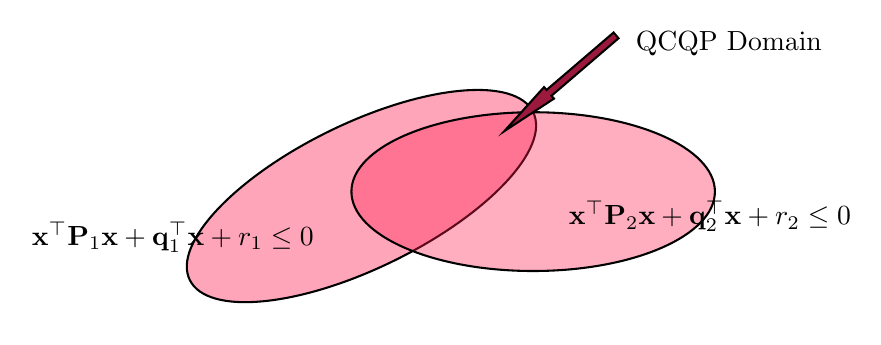
\begin{tikzpicture}[x=0.75pt,y=0.75pt,yscale=-0.75,xscale=0.75]
%uncomment if require: \path (0,300); %set diagram left start at 0, and has height of 300

%Shape: Ellipse [id:dp9898126968799086] 
\draw  [fill=mypink  ,fill opacity=0.4 ] (103.44,199.35) .. controls (92.18,176.27) and (132.43,133.45) .. (193.35,103.71) .. controls (254.27,73.97) and (312.79,68.57) .. (324.06,91.65) .. controls (335.32,114.73) and (295.07,157.55) .. (234.15,187.29) .. controls (173.23,217.03) and (114.71,222.43) .. (103.44,199.35) -- cycle ;
%Shape: Ellipse [id:dp5973223095827915] 
\draw  [fill=mypink  ,fill opacity=0.36 ] (207.31,142.65) .. controls (207.31,114.48) and (259.58,91.65) .. (324.06,91.65) .. controls (388.54,91.65) and (440.81,114.48) .. (440.81,142.65) .. controls (440.81,170.82) and (388.54,193.65) .. (324.06,193.65) .. controls (259.58,193.65) and (207.31,170.82) .. (207.31,142.65) -- cycle ;
%Left Arrow [id:dp11071847750004182] 
\draw  [fill=mydarkpink  ,fill opacity=1 ] (305.5,103.83) -- (331.05,75.5) -- (332.64,77.36) -- (375.73,40.44) -- (378.91,44.15) -- (335.82,81.07) -- (337.41,82.92) -- cycle ;

% Text Node
\draw (0,160) node [anchor=north west][inner sep=0.75pt]    {$\mathbf{x}^\top \mathbf{P}_1 \mathbf{x} + \mathbf{q}_1^\top\mathbf{x} + r_1 \leq 0$};
% Text Node
\draw (345,147) node [anchor=north west][inner sep=0.75pt]    {$\mathbf{x}^\top \mathbf{P}_2 \mathbf{x} + \mathbf{q}_2^\top\mathbf{x} + r_2 \leq 0$};
% Text Node
\draw (388,38) node [anchor=north west][inner sep=0.75pt]   [align=left] {QCQP Domain};


\end{tikzpicture}

\end{center} 
% \caption{Visualization of trajectory generation done in the developed software}
\end{figure}

 
\end{flushleft}
\end{frame}




\begin{frame}{Convex piece-wise linear functions}
\framesubtitle{Solution as LP}
\begin{flushleft}

We can formulate a minimization problem using convex piece-wise linear functions:

\begin{equation}
\begin{aligned}
& \underset{\mathbf{x}}{\text{minimize}}
& & \text{max}(\mathbf{a}_i^\top \mathbf{x} + b_i)
\end{aligned}
\end{equation}

\bigskip

Which can be equivalently transformed into the following LP:

\begin{equation}
\begin{aligned}
& \underset{\mathbf{x}, t}{\text{minimize}}
& & t \\
& \text{subject to}
& & \mathbf{a}_i^\top \mathbf{x} + b_i \leq t
%
\end{aligned}
\end{equation}

We can observe that optimal (minimal) $t$ will have to lie on one of the linear functions $\mathbf{a}_i^\top \mathbf{x} + b_i$, i.e. on the original piece-wise linear function $f(\mathbf{x})$. And optimal value on t corresponds to the smallest value of the original function $f(\mathbf{x})$.
 
\end{flushleft}
\end{frame}



\begin{frame}{Sum of piece-wise linear functions}
\framesubtitle{Solution as LP}
\begin{flushleft}


Sum of convex piece-wise linear functions have the form:

\begin{equation}
    f(\mathbf{x}) + g(\mathbf{x}) = \text{max}(\mathbf{a}_i^\top \mathbf{x} + b_i) +  \text{max}(\mathbf{c}_i^\top \mathbf{x} + d_i)
\end{equation}

\bigskip

Their representation as LP is:

\begin{equation}
\begin{aligned}
& \underset{\mathbf{x}, t_1, t_2}{\text{minimize}}
& & t_1 + t_2 \\
& \text{subject to}
& & \begin{cases}
\mathbf{a}_i^\top \mathbf{x} + b_i \leq t_1 \\
\mathbf{c}_i^\top \mathbf{x} + d_i \leq t_2
\end{cases}
%
\end{aligned}
\end{equation}


 
\end{flushleft}
\end{frame}




\begin{frame}{Convex piece-wise linear functions}
\framesubtitle{Code}
\begin{flushleft}

\begin{lstlisting}[language=Matlab]
n = 7; A = randn(n, n) - 3*rand*eye(n);
Q = eye(n);

cvx_begin sdp
    variable P(n, n) symmetric
    minimize 0
    subject to
        P >= 0;
        A'*P + P*A + Q <= 0;
cvx_end

if strcmp(cvx_status, 'Solved')
    [eig(A), eig(A*P + P*A' + Q), eig(P)]
else
    eig(A)
end
\end{lstlisting}
 
\end{flushleft}
\end{frame}



%\begin{frame}{Zero-infinity function}
%%	\framesubtitle{Code}
%	\begin{flushleft}
%		
%		Consider a function that returns 0 for negative inputs, and infinity for positive ones:
%		
%		\begin{equation}
%			f(x) = 
%			\begin{cases}
%				0 &x \leq 0 \\
%				\infty &x > 0
%			\end{cases}
%		\end{equation}
%	
%		We can equivalently replace it with the following piece-wise linear function:
%		
%		\begin{equation}
%			f(x) = 
%			\underset{\lambda \geq 0}{\text{max}}  \  \lambda x
%		\end{equation}		
%		
%	\end{flushleft}
%\end{frame}



\begin{frame}{Chebyshev center of a polyhedron}
\framesubtitle{Problem statement}
\begin{flushleft}

Chebyshev center of a polyhedron is the center of the largest ball inscribed in a polyhedron:

\begin{figure} [h!]
\begin{center}

% \tikzset{every picture/.style={line width=0.75pt}} %set default line width to 0.75pt        

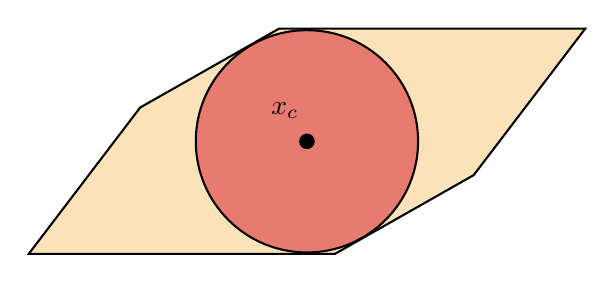
\begin{tikzpicture}[x=0.75pt,y=0.75pt,yscale=-0.7,xscale=0.7]
%uncomment if require: \path (0,300); %set diagram left start at 0, and has height of 300

%Snip Diagonal Corner Rect [id:dp285744847982357] 
\draw  [fill={rgb, 255:red, 245; green, 166; blue, 35 }  ,fill opacity=0.32 ] (286.75,53) -- (497.5,53) -- (497.5,53) -- (420.8,153.75) -- (325.25,208) -- (114.5,208) -- (114.5,208) -- (191.2,107.25) -- cycle ;
%Shape: Circle [id:dp4209627583449631] 
\draw  [fill={rgb, 255:red, 208; green, 2; blue, 27 }  ,fill opacity=0.46 ] (229.5,130.5) .. controls (229.5,88.25) and (263.75,54) .. (306,54) .. controls (348.25,54) and (382.5,88.25) .. (382.5,130.5) .. controls (382.5,172.75) and (348.25,207) .. (306,207) .. controls (263.75,207) and (229.5,172.75) .. (229.5,130.5) -- cycle ;
%Shape: Circle [id:dp17296463065051126] 
\draw  [fill={rgb, 255:red, 0; green, 0; blue, 0 }  ,fill opacity=1 ] (301.38,130.5) .. controls (301.38,127.95) and (303.45,125.88) .. (306,125.88) .. controls (308.55,125.88) and (310.63,127.95) .. (310.63,130.5) .. controls (310.63,133.05) and (308.55,135.13) .. (306,135.13) .. controls (303.45,135.13) and (301.38,133.05) .. (301.38,130.5) -- cycle ;

% Text Node
\draw (279.33,101.67) node [anchor=north west][inner sep=0.75pt]   [align=left] {$\displaystyle x_{c}$};


\end{tikzpicture}
\end{center} 
% \caption{Visualization of trajectory generation done in the developed software}
\end{figure}

Equation describing this ball can be written as:

\begin{equation}
    \mathcal{B} = \{ \mathbf{x}_c + \mathbf{u}: \ ||\mathbf{u}||_2 \leq r \}
\end{equation}

where $r$ is the radius of the ball and $\mathbf{x}_c$ is its center.
 
\end{flushleft}
\end{frame}



\begin{frame}{Chebyshev center of a polyhedron}
	\framesubtitle{Max over the dot product}
	\begin{flushleft}
		
		Before we move towards solving the problem, let us consider the following maximization: 
		
		\begin{equation}
			\text{sup} \{ \mathbf{a}^\top \mathbf{u}: \ ||\mathbf{u}||_2 \leq r \}
		\end{equation}
	
	We can re-write the expression:
	
		\begin{equation}
			\text{sup} \{ \mathbf{a}^\top \mathbf{u}: \ ||\mathbf{u}||_2 \leq r \}  = 
			\text{sup} \{ ||\mathbf{a}|| \cdot ||\mathbf{u}|| \text{cos}(\varphi): \ ||\mathbf{u}||_2 \leq r \}
		\end{equation}
%	
where $\varphi$ is the angle between $\mathbf{a}$ and $\mathbf{u}$. Since $\mathbf{a}$ is constant, $\text{max}(||\mathbf{u}||) = r$, and $\text{max}(\text{cos}(\varphi)) = 1$, we get:
	
	\begin{equation}
		\text{sup} \{ \mathbf{a}^\top \mathbf{u}: \ ||\mathbf{u}||_2 \leq r \}  = 
		 ||\mathbf{a}|| r
	\end{equation}
	
		
	\end{flushleft}
\end{frame}




\begin{frame}{Chebyshev center of a polyhedron}
\framesubtitle{Solution as LP, part one}
\begin{flushleft}

For the ball $\mathcal{B}$ to be inscribed in a polygon $\mathcal{P} = \{ \mathbf{x}: \ \mathbf{A}\mathbf{x} \leq \mathbf{b} \}$, the following should hold:

\begin{equation}
    \text{sup} \{ \mathbf{a}_i^\top (\mathbf{x}_c + \mathbf{u}): \ ||\mathbf{u}||_2 \leq r \} \leq b_i
\end{equation}

Note that the largest value of $\mathbf{a}_i^\top \mathbf{u}$ under condition $||\mathbf{u}||_2 \leq r$ is $r ||\mathbf{a}_i||$: it can indeed achieve this value if $\mathbf{a}_i$ and $\mathbf{u}$ are co-directional, but a larger one is not possible. Therefore:

\begin{equation}
    \text{sup} \{ \mathbf{a}_i^\top (\mathbf{x}_c + \mathbf{u}): \ ||\mathbf{u}||_2 \leq r \}  = 
    \mathbf{a}_i^\top \mathbf{x}_c + r ||\mathbf{a}_i||
    \leq b_i
\end{equation}

 
\end{flushleft}
\end{frame}



\begin{frame}{Chebyshev center of a polyhedron}
\framesubtitle{Solution as LP, part two}
\begin{flushleft}

Finally, we can write down the solution of the problem as a linear optimization:

\begin{equation}
\begin{aligned}
& \underset{r, \ \mathbf{x}_c}{\text{maximize}}
& & r \\
& \text{subject to}
& & \mathbf{a}_i^\top \mathbf{x}_c + r ||\mathbf{a}_i||
    \leq b_i
%
\end{aligned}
\end{equation}

 
\end{flushleft}
\end{frame}




\begin{frame}{Chebyshev center of a polyhedron}
\framesubtitle{Code}
\begin{flushleft}

Below we can see MATLAB code for solving the problem:

\begin{lstlisting}[language=Matlab]
n = 7; A = 0.35*randn(n, n);
Q = eye(n);

cvx_begin sdp
    variable P(n, n) symmetric
    minimize 0
    subject to
        P >= 0;
        A'*P*A - P + Q <= 0;
cvx_end

if strcmp(cvx_status, 'Solved')
    [abs(eig(A)), eig(A'*P*A - P), eig(P)]
else
    abs(eig(A))
end
\end{lstlisting}

 
\end{flushleft}
\end{frame}




\begin{frame}{Linear-Fractional Programming}
%	\framesubtitle{Formulation}
	\begin{flushleft}
		
		The following is the Linear-Fractional Programming problem:
		
		\begin{equation}
			\begin{aligned}
				& \underset{\mathbf{x}}{\text{maximize}}
				& & \frac{\mathbf{c}^\top \mathbf{x} + d}{\mathbf{e}^\top \mathbf{x} + f} \\
				& \text{subject to}
				& & 
				 \begin{cases}
				 	\mathbf{A} \mathbf{x} \leq \mathbf{b} \\
				 	\mathbf{A}_e \mathbf{x} = \mathbf{b}_e
				 \end{cases}
			\end{aligned}
		\end{equation}
		
		This doesn't look like an LP, but let us see if we can try to bring the problem to the LP form. 
		
	\end{flushleft}
\end{frame}



\begin{frame}{Linear-Fractional Programming}
%	\framesubtitle{LP form}
	\begin{flushleft}
		
		The following is the Linear-Fractional Programming problem in LP form:
		
		\begin{equation}
			\begin{aligned}
				& \underset{\mathbf{y}, \ z}{\text{maximize}}
				& & \mathbf{c}^\top \mathbf{y} + z d \\
				& \text{subject to}
				& & 
				\begin{cases}
					\mathbf{A} \mathbf{y} \leq z \mathbf{b} \\
					\mathbf{A}_e \mathbf{y} = z \mathbf{b}_e \\
					\mathbf{e}^\top \mathbf{y} + z f = 1 \\
					z \geq 0
				\end{cases}
			\end{aligned}
		\end{equation}
		
		Here the variables $\mathbf{y}$ and $z$ are related to $\mathbf{x}$ as follows.
		
		\begin{equation}
			\mathbf{y} = \frac{\mathbf{x}}{\mathbf{e}^\top \mathbf{x} + f}
		\end{equation}
	 
		\begin{equation}
			z = \frac{1}{\mathbf{e}^\top \mathbf{x} + f}
		\end{equation} 
		
	\end{flushleft}
\end{frame}



\begin{frame}{Linear-Fractional Programming}
%	\framesubtitle{details}
	\begin{flushleft}
		
		We assumed that the domain of the previous problem is limited to $\mathbf{e}^\top \mathbf{x} + f \geq 0$. With that we have:
		
		\begin{equation}
			 \mathbf{c}^\top \mathbf{y} + z d 
			 = 
			 \mathbf{c}^\top\frac{\mathbf{x}}{\mathbf{e}^\top \mathbf{x} + f} + \frac{1}{\mathbf{e}^\top \mathbf{x} + f} d 
			 =
			 \frac{\mathbf{c}^\top\mathbf{x} + d}{\mathbf{e}^\top \mathbf{x} + f}
		\end{equation}
		
		
		\begin{equation}
			\mathbf{A} \mathbf{y} \leq z \mathbf{b} 
			\implies
			\mathbf{A} \frac{\mathbf{x}}{\mathbf{e}^\top \mathbf{x} + f} \leq \frac{1}{\mathbf{e}^\top \mathbf{x} + f} \mathbf{b} 
			\implies
			\mathbf{A} \mathbf{x} \leq \mathbf{b} 
		\end{equation}
		
		
	\end{flushleft}
\end{frame}





\begin{frame}{Homework}
% \framesubtitle{Parameter estimation}
\begin{flushleft}

Implement linear approximation of a convex function and solve it as LP

\end{flushleft}
\end{frame}





\begin{frame}{Further reading}
	% \framesubtitle{Parameter estimation}
	\begin{flushleft}
		
		\bref{https://fmin.xyz/docs/methods/Simplex.html}{Linear Programming and simplex algorithm}, fmin.
		
	\end{flushleft}
\end{frame}






\myqrframe


\end{document}
